\subsubsection{Bild-basierte Rechnungsklassifizierung}
\label{chap:image-recon}
% http://citeseerx.ist.psu.edu/viewdoc/download?doi=10.1.1.414.9846&rep=rep1&type=pdf

% Analog der Klassifizierung von Objekten auf Fotos, ist es auch denkbar, Rechnung mit Hilfe diesem Bild-basiertem Vorgehen zu klassifizieren.

Wie im vorherigen Kapitel erwähnt, ist die Klassifizierung von Bildern eine bekannte Problematik aus dem Bereich der Computer-Vision. Dieses Kapitel widmet sich einem Experiment, bei welchem Algorithmen und Modelle aus dem Bereich der Computer-Vision angewendet werden, um Rechnungen zu klassifizieren.

Auf dem Machine Learning Blog \enquote{Towards Data Science} beschreiben und vergleichen diverse Autoren verschiedenste Modelle im Bereich der Computer Vision. Der Blog bietet einen guten Überblick über die aktuellen Methoden zur Klassifizierung von Bildern. So werden im Juli 2017 die Residual Networks (kurz ResNet), entwickelt von \textcite{He2015}, als die bahnbrechendse Eingabe beim ImageNet LSVRC Wettbewerb\footnote{Die ImageNet Large Scale Visiual Recognition Competition (LSVRC) ist ein Wettbewerb der ImageNet Organisation, bei welcher hunderte Data Scientists ihre Modelle im Bereich der Computer Vision vergleichen.} der letzten Jahre bezeichnet~\autocite{Fungg2017ResNet}. Im September 2018 beschreibt \textcite{SHTsuang2018Inception} das InceptionV4 Netzwerk von Google, welches vom GoogLeNet abgeleitet und mit den Ideen aus dem ResNet erweitert wurde. Das Modell erzielt noch bessere Resultate als das ResNet selbst. Im gleichen Artikel wird auch das Inception-ResNet-V2 vorgestellt, welches im Vergleich zum InceptionV4 Netzwerk schneller trainiert werden kann und zugleich etwas bessere Resultate erzielt. 

In einem Blog Post auf dem Google AI Blog präsentieren Forscher aus dem Google Brain Team das NASNet. NASNet ist ein Modell zur Klassifizierung von Bildern, welches durch die Anwendung von Machine Learning designed wurde~\autocite{GoogleNasNet}. Unter dem Codename AutoML publiziert das Google Brain Team einen Ansatz, bei welchem ein Neuronales Netzwerk ein anderes erstellt - eine künstliche Intelligenz, welche eine neue künstliche Intelligenz schafft. Mit diesem Ansatz kann das sehr aufwendige Design eines Neuronalen Netzwerks vereinfacht beziehungsweise automatisiert werden~\autocite{GoogleAutoML}.


Als Teil des selben Blog Posts, in welchem das NASNet präsentiert wird, vergleichen die Forscher von Google das Modell mit anderen Netzwerken, wie dem ResNet und dem Inception-ResNet-V2. Der Abbildung \ref{nasnet-comparision} ist zu entnehmen, dass das vom Google Brain Team präsentierte NASNet, in der \enquote{medium} Ausprägung, trotz reduzierter Anzahl an benötigter Operationen, sprich reduzierter Komplexität, eine verbesserte Treffergenauigkeit als die bisherigen Netzwerke erzielt. In der \enquote{large} Ausprägung kann das NASNet durch eine erhöhte Komplexität eine noch bessere Treffergenauigkeit erzielen~\autocite{GoogleNasNet}.

\begin{figure}[h]
% \begin{wrapfigure}{r}{0.6\textwidth} 
    \captionsetup{width=.9\linewidth}
    \caption[Vergleich des NASNet mit anderen Netzwerken zur Klassifizierung von Bildern]{Vergleich des vom Google Brain Team präsentierten NASNet mit älteren Netzwerken zur Klassifizierung von Bildern des ImageNet Datensatzes. Es wird die Treffergenauigkeit, der Prozentsatz richtig Klassifizierter Bilder der Gesamtheit aller Bilder, der Anzahl benötigter Operationen, sprich die Komplexität des Netzwerks, gegenübergestellt.}
    \label{nasnet-comparision}
    \centering
    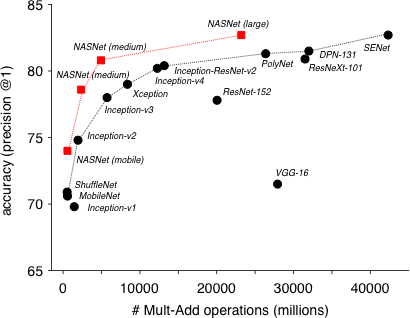
\includegraphics[width=0.55\textwidth]{graphics/nasnet-comparision.jpg}
    \caption*{Quelle: \textcite{GoogleNasNet}}
\end{figure}
%\end{wrapfigure}

% ResNet Arxiv: https://arxiv.org/abs/1512.03385
% ResNet: https://towardsdatascience.com/an-overview-of-resnet-and-its-variants-5281e2f56035
% DRM Arxiv: https://arxiv.org/abs/1512.03385
% DRN: https://towardsdatascience.com/review-drn-dilated-residual-networks-image-classification-semantic-segmentation-d527e1a8fb5
% InceptionV4: https://towardsdatascience.com/review-inception-v4-evolved-from-googlenet-merged-with-resnet-idea-image-classification-5e8c339d18bc

% NASNet: https://ai.googleblog.com/2017/11/automl-for-large-scale-image.html

% NASNet example https://www.tensorflow.org/hub/tutorials/image_retraining

% AutoML: https://ai.googleblog.com/2017/05/using-machine-learning-to-explore.html


% TODO: Dilated Residual Network beschreiben: Veränderung der Convolutions in einem ResNet zu einem Grid anstelle der herkömmlichen convolution.

Im folgenden wird das ResNet, das Inception-ResNet-V2 sowie das NASNet large Netzwerk angewendet, um die bisher bei der AXA eingereichten Rechnung zu klassifizieren.

Um Bilderkennungsmodelle mit Millionen von Parametern zu trainieren, werden viele Trainingsdaten und eine enorme Kapazität an Rechenleistung benötigt. Das Konzept des Transfer Learning bietet die Möglichkeit, diese beiden Problematiken zu Umgehen und dabei nur wenig oder keine Treffergenauigkeit einzubüssen (vgl. Kapitel \ref{chap:transfer-learning})~\autocite{TDSTransferLearning}. % \autocite{TensorflowImageRetraining}

Um die Rechnungen zu klassifizieren wird Transfer Learning angewendet, indem die genannten Modelle auf dem ImageNet Datensatz trainiert werden, bevor die eigentliche Problemstellung angegangen wird.

Nach dem Training auf dem ImageNet Datensatz werden die letzten Schichten des Netzwerks, jene die für die Klassifizierung zuständig sind, durch ein neues Klassifizierungsnetzwerk ersetzt. Dadurch wird der Trainingseffekt durch den ImageNet Datensatz beibehalten und die Klassifizierung so angepasst, dass sie die Einteilung in die vier vorliegenden Klassen erlaubt.

Das Klassifizierungsnetzwerk (vgl. Abbildung \ref{image-classification-model}), welches zur Anwendung kommt, besteht aus einem Convolution Layer sowie drei Fully Connected Layer\footnote{Ein Fully Connected Layer ist die einfachste Schicht eines neuronalen Netzwerks. Die Schicht besteht aus einer variablen Anzahl an Neuronen (vgl. Kapitel \ref{chap:neuron}). Jedes einzelne Neuron ist mit allen Neuronen der vorhigen Schicht verbunden. Ein Beispiel einer solchen Schicht ist im Kapitel \ref{chap:deep-neural-nets} zu sehen.}. Zwischen den Fully Connected Layern sind zwei Dropout Layer zur Reduzierung des Overfitting eingeschoben. Im Falle des NASNet entfällt der Convolution Layer, da das Netzwerk bereits einen eindimensionalen Feature-Vektor als Ausgabe liefert.


\begin{figure}[h!] 
  \captionsetup{width=.9\linewidth}
  \caption[Neuronale Netze, welche bei der Bild-basierten Klassifizierung zur Anwendung kommen]{Neuronale Netze, welche bei der Bild-basierten Klassifizierung zur Anwendung kommen. Input ist jeweils der Feature-Vektor, welcher durch das ResNet, Inception-ResNet beziehungsweise NASNet Netzwerk erstellt wurde. Beim ResNet und Inception-ResNet wird dieser Feature-Vektor durch ein 2D-Convolution und ein Flatten Layer in einen eindimensionalen Vektor gebracht. Das NASNet liefert bereits einen eindimensionalen Feature-Vektor und die ersten zwei Schichten fallen somit weg. Durch zwei Hidden Layer wird der Vektor schlussendlich zu einem One-Hot Encoded Vektor für die vier Klassen reduziert.}
  \label{image-classification-model} 
  \begin{subfigure}[b]{0.3\linewidth}
    \centering
    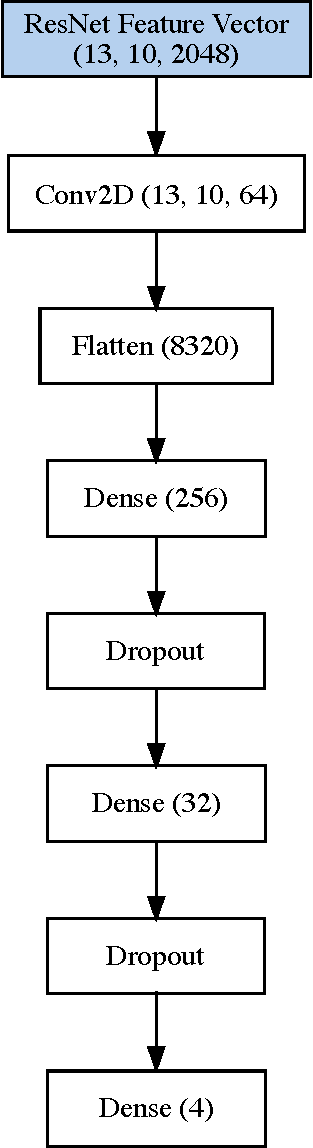
\includegraphics[scale=0.6]{graphics/image-classification-results/model/resnet.pdf} 
    \caption{ResNet} 
    \label{image-classification-model:resnet} 
    \vspace{2ex}
  \end{subfigure}%% 
   \begin{subfigure}[b]{0.3\linewidth}
    \centering
    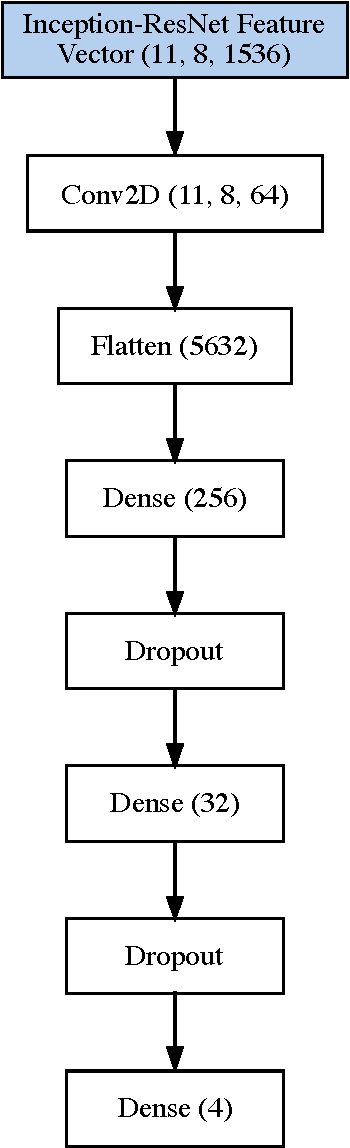
\includegraphics[scale=0.6]{graphics/image-classification-results/model/inception.pdf} 
    \caption{Inception-ResNet-V2} 
    \label{image-classification-model:inception} 
    \vspace{2ex}
  \end{subfigure}%% 
  \begin{subfigure}[b]{0.3\linewidth}
    \centering
    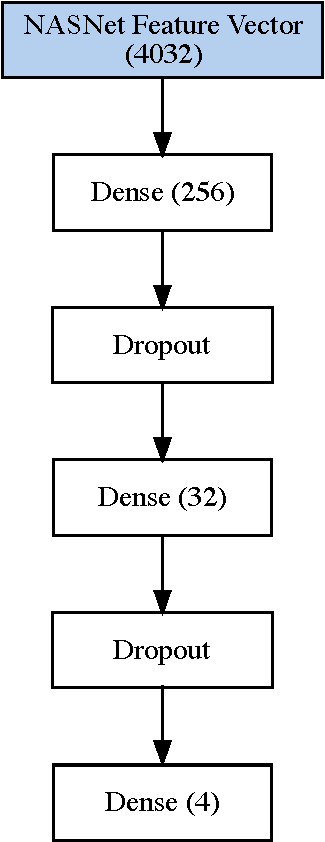
\includegraphics[scale=0.6]{graphics/image-classification-results/model/nasnet.pdf} 
    \caption{NASNet} 
    \label{image-classification-model:nasnet} 
    \vspace{2ex}
  \end{subfigure} 
  \centering
\end{figure}

Die genannten Modelle werden mit 80\% der vorhandenen Daten trainiert, die übrigen 20\% werden benötigt, um den Trainingsfortschritt zu prüfen. Mit diesen 20\% Testdaten soll ein allfälliges Overfitting erkannt werden.

Die Abbildung \ref{image-class-results} zeigt das Training der genannten Modelle während 60 Trainingsepochen (Trainingseinheiten). \ref{image-class-results:a} und \ref{image-class-results:b} zeigen die Treffergenauigkeit respektive das loss während dem Training.  \ref{image-class-results:c} und \ref{image-class-results:d} zeigen die Treffergenauigkeit respektive das loss bei der Anwendung des Modells auf den Testdaten. 

\begin{figure}[h!] 
  \captionsetup{width=.9\linewidth}
  \caption[Statistiken aus dem Training der Bild-basierten Klassifizierung von Rechnungen]{Statistiken aus dem Training der Bild-basierten Klassifizierung von Rechnungen mit den ResNet, Inception-ResNetV2 und NASNet Netzwerken.}
  \label{image-class-results} 
  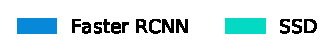
\includegraphics[scale=1]{graphics/matplot/img-detection__legend_1.pdf}
  \begin{subfigure}[b]{0.5\linewidth}
    \centering
    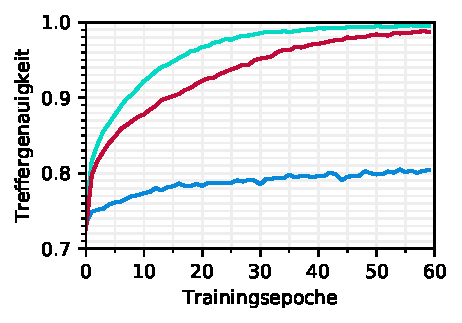
\includegraphics[scale=1]{graphics/matplot/img-class__acc.pdf}
    \caption{Treffergenauigkeit} 
    \label{image-class-results:a} 
    \vspace{2ex}
  \end{subfigure}%% 
  \begin{subfigure}[b]{0.5\linewidth}
    \centering
    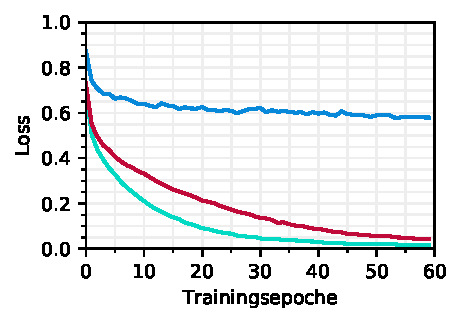
\includegraphics[scale=1]{graphics/matplot/img-class__loss.pdf}
    \caption{loss} 
    \label{image-class-results:b} 
    \vspace{2ex}
  \end{subfigure} 
  \begin{subfigure}[b]{0.5\linewidth}
    \centering
    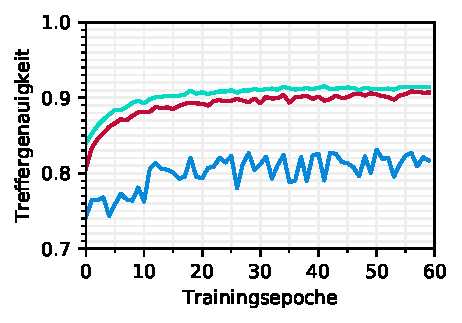
\includegraphics[scale=1]{graphics/matplot/img-class__val_acc.pdf}
    \caption{Treffergenauigkeit bei den Testdaten} 
    \label{image-class-results:c} 
  \end{subfigure}%%
  \begin{subfigure}[b]{0.5\linewidth}
    \centering
    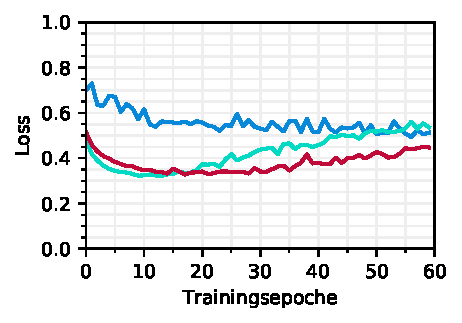
\includegraphics[scale=1]{graphics/matplot/img-class__val_loss.pdf}
    \caption{loss bei den Testdaten} 
    \label{image-class-results:d} 
  \end{subfigure}
  \centering
\end{figure}

% Die einzelnen Modelle zeigen eine Treffergenauigkeit von TODO\% (ResNet, Epoche TODO), TODO\% (Inception-ResNet-V2, Epoche TODO) beziehungsweise TODO\% (NASNet, Epoche TODO).

% Das auf dem TODO TODO TODO\todo{TODO} basierende Modell hat mit einer Treffergenauigkeit von \todo{TODO}\% nach \todo{TODO} Epochen die höchste Treffergenauigkeit auf den Testdaten. 

Auffällig ist das schlechte Resultate des NASNet Modells. Obwohl das NASNet als eines der genausten Klassifizierungsmodelle für Bilder gilt, schneidet es im vorliegenden Experiment mit Abstand am schlechtesten ab. Auffällig ist auch, dass die Treffergenauigkeit auf dem Testdatensatz sehr sprunghaft ist.

Eine fundierte Erklärung, weshalb das NASNet Modell so schlecht abschneidet, kann nicht gefunden werden. Eine mögliche Erklärung ist der mit Abstand kleinere Feature-Vektor des NASNets. Dieser ist mit nur 4032 Neuronen wesentlich kleiner als jener des ResNet (266240 Neuronen) und des Inception-ResNet-V2 (135168 Neuronen).

Die Ergebnisse des ResNet und des Inception-ResNet-V2 sehen dagegen wesentlich besser aus. Während dem Training steigt die Treffergenauigkeit stetig an und das loss sinkt stetig. Die Modelle weisen bereits nach 30 Epochen einen Bias von weniger als 5\% (ResNet) respektive weniger als 2\% (Inception-ResNet-V2) auf. Nach 60 Epochen Training weisen die beiden Modelle einen Bias von weniger als 1.5\% respektive 0.5\% auf. Dies zeigt, dass die gewählten Modelle lernen und grundsätzlich geeignet sind, die Problemstellung anzugehen. 

Neben der auch nach 60 Epochen noch leicht steigenden Treffergenauigkeit hat das loss auf den Testdaten (vgl. Abbildung \ref{image-class-results:d}) bereits nach 25 (ResNet) respektive 15 (Inception-ResNet-V2) Epochen den Wendepunkt erreicht. Dies zeigt, dass das Modell zu wenig gut Generalisiert. Die steigende Testgenauigkeit vermittelt zwar einen guten eindruck, das steigende loss zeigt jedoch, dass das Modell in seinen Entscheidungen immer unsicherer wird, das heisst die Wahrscheinlichkeit, mit welcher sich das Modell sicher ist, eine Rechnung einer bestimmten Klasse zuzuweisen, sinkt. Das Modell beginnt also nach nur wenigen Epochen Auswendig zu lernen (Overfitting).

Das Problem des Overfitting könnte womöglich durch zusätzliche Trainingsdaten gemindert werden, diese stehen jedoch nicht zur Verfügung.

Konkludierend kann gesagt werden, dass durch den Bild-basierten Ansatz eine Klassifizierung möglich ist, aktuell aber zu wenig Testdaten zur Verfügung stehen, um den Ansatz weiter zu verfolgen.

Im folgenden Kapitel wird ein weiterer Ansatz zur Klassifizierung der Rechnungen gezeigt, welcher mit den vorhandenen Datensätzen bessere Ergebnisse erzielen kann.

% Optimierungspotential:

% - https://towardsdatascience.com/deep-learning-performance-cheat-sheet-21374b9c4f45

% ENAS: https://github.com/carpedm20/ENAS-pytorch
% Neural Architecture Search with Reinforcement Learning: https://arxiv.org/abs/1611.01578
% Neural Optimizer Search with Reinforcement Learning: https://arxiv.org/abs/1709.07417

% \textbf{Weight penalty L1 and L2}
% Improve performance and reduce overfitting -> Keeps weights in NN small
% -> Have a look at the trained model, are there huge weights? If so, highlight this as a problem


